\documentclass[12pt,a4paper,UTF8]{article}
% \usepackage{ctex} % Chinese support
\usepackage{graphicx} % Insert images
\usepackage{listings} % Print source code
\usepackage{color} % Color support
\usepackage{booktabs} % Professional table support
\usepackage{pdflscape} % Landscape pages support in PDF
\usepackage{hyperref} % Hypertext links support for cross-referencing

% Customize hyperref format (it's set to no special format here)
\hypersetup{hidelinks}

% Declare directories to search for graphics files for graphicx
\graphicspath{{figures/}{logo/}}

% Define source code style for listings
\lstdefinestyle{python}{
  language=Python,
  basicstyle=\ttfamily\footnotesize,
  keywordstyle=\bfseries\color[rgb]{0, 0, 1},
  identifierstyle=\color[rgb]{0.5, 0.3, 0.1},
  stringstyle=\color[rgb]{0.6, 0.1, 0.1},
  commentstyle=\itshape\color[rgb]{0.05, 0.5, 0.05},
  backgroundcolor=\color[gray]{0.95},
  numbers=left,
  numbersep=5pt,
  numberstyle=\color[gray]{0.6},
  breaklines=true
}

% Define new command for title page
\newcommand{\reporttitle}[2]{
  \LARGE\textsf{#1}\quad\underline{\makebox[12em]{#2}}
}
\newcommand{\reportinfo}[2]{
  \large\makebox[4em]{\textsf{#1}}\quad\underline{\makebox[18em]{#2}}
}

% The document begins here
\begin{document}
\begin{titlepage}
  \centering
  \vspace*{\fill}
  
\includegraphics[height=144pt]{nju-logo}\\[48pt]
  {\huge\textsf{Lab Report}}\\[48pt]
  \reporttitle{Lab Name}{Content Delivery Network}\\[72pt]

  \reportinfo{Course}{Computer Network}\\[8pt]
  \reportinfo{Major}{Computer Science and Technology}\\[8pt]
  \reportinfo{Id}{191220129}\\[8pt]
  \reportinfo{Name}{Shangyu.Xing}\\[8pt]
  \reportinfo{Email}{191220129@smail.nju.edu.cn}\\[8pt]
  \reportinfo{Date}{2021.06}\\
  \vspace*{\fill}
\end{titlepage}

\tableofcontents
\newpage

\section{Objective}
\begin{itemize}
	\item Learn CDN and how to implement it;
	\item Get to know real network by deploying code to physical servers.
\end{itemize}

\section{Requirements}
	This lab requires to implement a simplified dns server and caching server to achieve CDN.
\begin{itemize}
	\item DNS server:
	\subitem Load DNS records table;
	\subitem reply DNS requests from client.
	\item caching server:
	\subitem reply GET requests from client;
	\subitem fetch files from remote server;
	\subitem maintain cache table.
\end{itemize}

\section{Procedure}
I completed all the tasks as required \textbf{including the optional task}.
In this section, I will explain how I did my work in detail.

\subsection{DNS Server}
\subsubsection{Load DNS Records Table}
Just read the file and store the information into a list object for further querying. The method 'str.split' can convert a string to a list.
\lstinputlisting[style=python]{1.py}

\subsubsection{Match Domain}
When the dns server receives a request from client, it should match the requested domain with the records table stored.
Note that the table contains entry with * as beginning (which means the it can be matched with anything).
However in this case it seems like a bit of overkill to use regular expression, so I adopted a policy to match the two string from end to beginning, and when the pointer moves to *, the match is successful.
\lstinputlisting[style=python]{2.py}

\subsubsection{Select the Nearest IP}
Simply traverse the matched ip list and select the nearest under Euclid distance.
\lstinputlisting[style=python]{3.py}

\subsection{Caching Server}
When the cache server receives a get request, it should do the following:
\begin{enumerate}
	\item check if the requested file is in cache;
	\item if not, fetch the file from remote server and store it in cache;
	\item return the file to the client.
\end{enumerate}
The first and second steps are implemented in touchItem, and the last step is implemented in do\_get.

\subsubsection{Do Get}
Do Get should also handle file not found error.
\lstinputlisting[style=python]{4.py}

\subsubsection{TouchItem}
\lstinputlisting[style=python]{5.py}

\subsubsection{Stream Forwarding}
The workflow is as follows:
\begin{enumerate}
	\item Upon receiving a request, the server search its cache for the requested file;
	\item if found, return the whole body to client;
	\item if not, fetch and send headers from remote server and repeat these steps until the whole body is received and sent:
	\subitem fetch 64KB data of body from remote server;
	\subitem send it to client.
\end{enumerate}
To complete stream forwarding, I create a bytearray buffer as a member variable of CacheServer, along with some variables indicating the current state. \\
I also created a method get\_body, which can be repeated called to get 64KB of body data. Every time it is called, it reads 64KB of response data into the buffer and return it. Note that the response object is stored as a member variable of CacheServer immediately after fetching and sending headers of the requested file.
\lstinputlisting[style=python]{6.py}
The method do\_GET should also be modified:
\lstinputlisting[style=python]{7.py}
But do\_HEAD remains the same since the headers are not streamed.

\section{Test \& Result}
\subsection{Testcases}
Firstly I tested my code using the given testcases.
\begin{figure}[htbp]
	\centering
	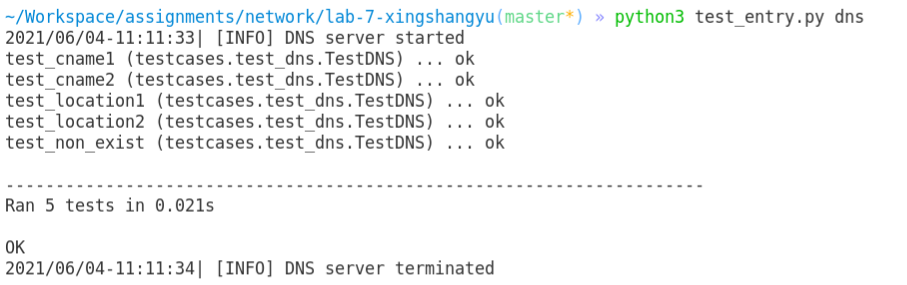
\includegraphics[width=\textwidth]{1}
	\caption{test dns}
\end{figure}
\begin{figure}[htbp]
	\centering
	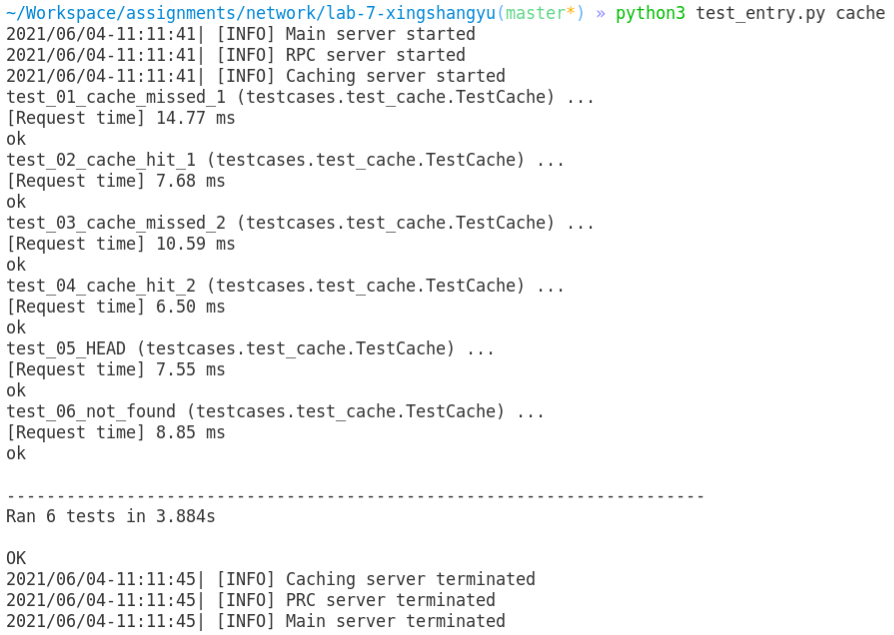
\includegraphics[width=\textwidth]{2}
	\caption{test cache}
\end{figure}
\begin{figure}[htbp]
	\centering
	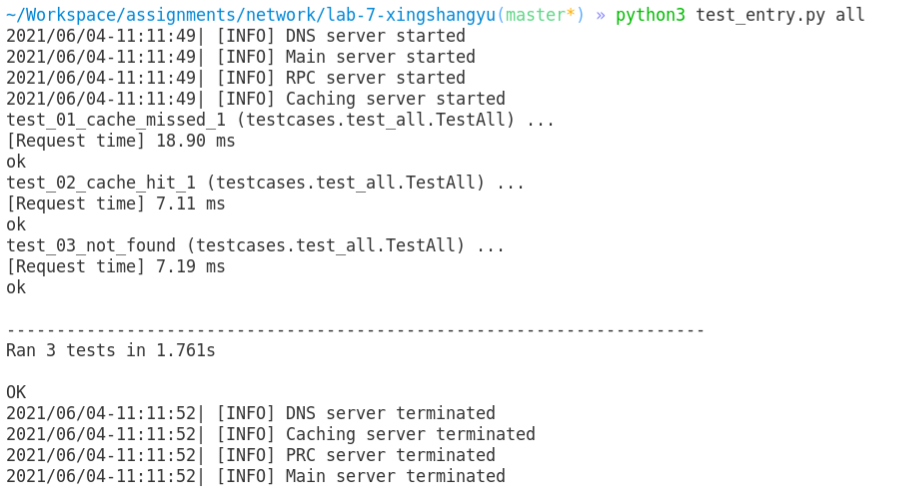
\includegraphics[width=\textwidth]{3}
	\caption{test all}
\end{figure}

\newpage
\subsection{Deployment}
The test log is here:
\begin{figure}[htbp]
	\centering
	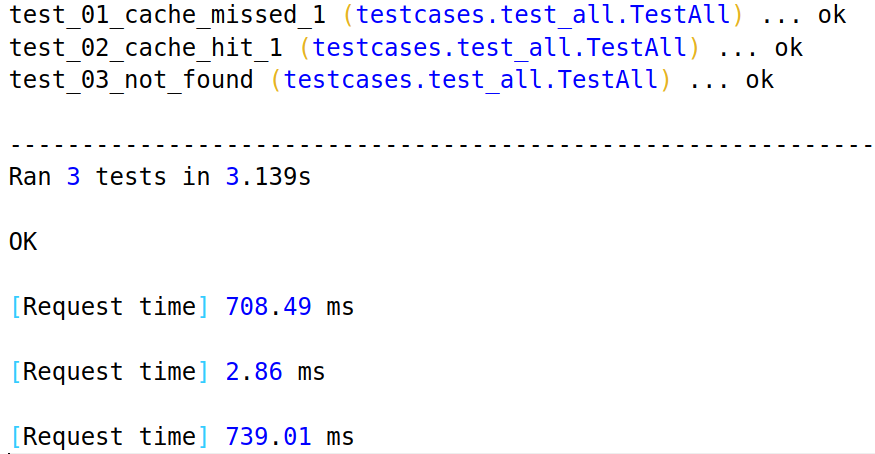
\includegraphics[width=\textwidth]{4}
	\caption{client log}
\end{figure}
\begin{figure}[htbp]
	\centering
	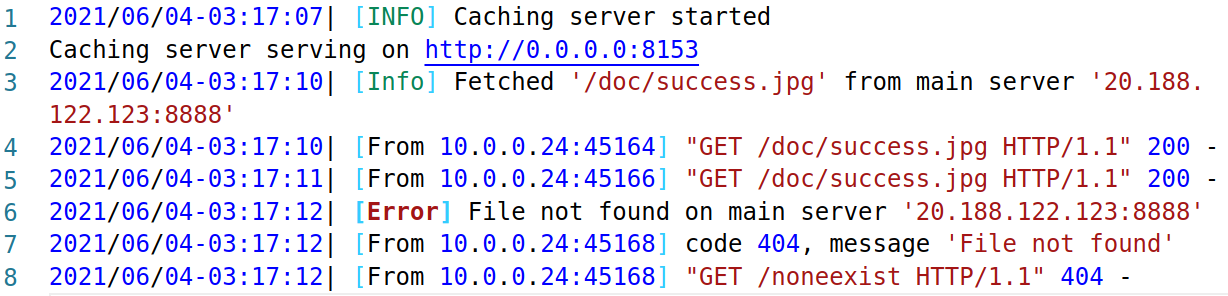
\includegraphics[width=\textwidth]{5}
	\caption{cache server log}
\end{figure}
\begin{figure}[htbp]
	\centering
	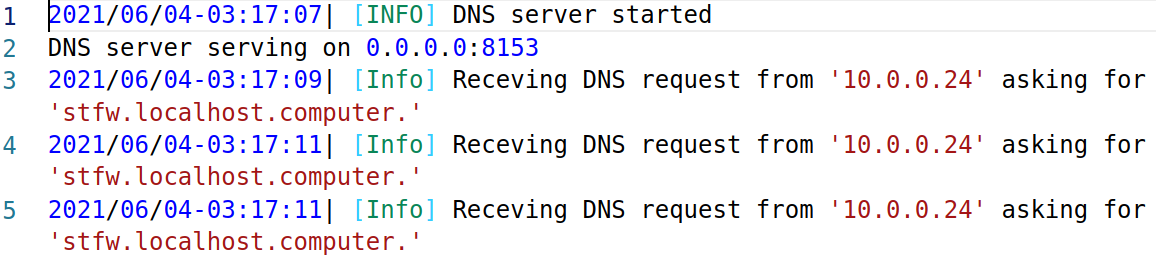
\includegraphics[width=\textwidth]{6}
	\caption{dns log}
\end{figure}
\newpage
Explanation:
\begin{itemize}
	\item In the first test the file was not cached, so caching server fetched the file from remote server, which consumed over 700ms.
	\item In the second test, the file had already been cached, so the server returned the file from its cache immediately, which consumed less than 3ms.
	\item In the first test the file was not cached, so caching server asked for the file from remote server and got a file not found error, which also consumed over 700ms.
\end{itemize}
We can learn that CDN greatly shorten the response time.

\section{Summary}
\begin{itemize}
	\item Knowing how to effectively use debugging tools such as pdb will greatly enhance working efficiency;
	\item English reading and writing skills are important.
\end{itemize}

\end{document}